\documentclass[12pt]{article}
\usepackage{amsthm,amssymb,amsmath,amsfonts}
\usepackage[a4paper, top=25mm, bottom=30mm, left=25mm, right=25mm]{geometry}
\usepackage[pagebackref=false,colorlinks,linkcolor=black,citecolor=black]{hyperref}
\usepackage[nameinlink]{cleveref}
 \AtBeginDocument{%
    \crefname{equation}{برابری}{equations}%
    \crefname{chapter}{فصل}{chapters}%
    \crefname{section}{بخش}{sections}%
    \crefname{appendix}{پیوست}{appendices}%
    \crefname{enumi}{مورد}{items}%
    \crefname{footnote}{زیرنویس}{footnotes}%
    \crefname{figure}{شکل}{figures}%
    \crefname{table}{جدول}{tables}%
    \crefname{theorem}{قضیه}{theorems}%
    \crefname{lemma}{لم}{lemmas}%
    \crefname{corollary}{نتیجه}{corollaries}%
    \crefname{proposition}{گزاره}{propositions}%
    \crefname{definition}{تعریف}{definitions}%
    \crefname{result}{نتیجه}{results}%
    \crefname{example}{مثال}{examples}%
    \crefname{remark}{نکته}{remarks}%
    \crefname{note}{یادداشت}{notes}%
    \crefname{observation}{مشاهده}{observations}%
    \crefname{algorithm}{الگوریتم}{algorithms}%
    \crefname{cproof}{برهان}{cproofs}%
}

\usepackage{tikz}
\usepackage{graphicx}
\usepackage{color}

\usepackage{setspace}
\doublespacing

\usepackage{titletoc}
\usepackage{tocloft}
\usepackage{enumitem}

\usepackage{algorithm}
% \usepackage[noend]{algpseudocode}
\usepackage[noend]{algorithmic}
\renewcommand{\algorithmicrequire}{\textbf{Input:}}
\renewcommand{\algorithmicensure}{\textbf{Output:}}

\usepackage{tabularx}
\makeatletter
\newcommand{\multiline}[1]{%
  \begin{tabularx}{\dimexpr\linewidth-\ALG@thistlm}[t]{@{}X@{}}
    #1
  \end{tabularx}
}
\makeatother

\usepackage{float}
\usepackage{verbatim}
\makeindex
\usepackage{sectsty}
\usepackage{xepersian}
\SepMark{-}
\settextfont[Scale=1.2,Path=fonts/,BoldFont=B Nazanin Bold.ttf]{B Nazanin.ttf}
\setlatintextfont{Times New Roman}
\renewcommand{\labelitemi}{$\bullet$}

\theoremstyle{definition}
\newtheorem{definition}{تعریف}[section]
\newtheorem{remark}[definition]{نکته}
\newtheorem{note}[definition]{یادداشت}
\newtheorem{example}[definition]{نمونه}
\newtheorem{question}[definition]{سوال}
\newtheorem{remember}[definition]{یاداوری}
\newtheorem{observation}[definition]{مشاهده}
\theoremstyle{theorem}
\newtheorem{theorem}[definition]{قضیه}
\newtheorem{lemma}[definition]{لم}
\newtheorem{proposition}[definition]{گزاره}
\newtheorem{corollary}[definition]{نتیجه}
\newtheorem*{cproof}{برهان}



\begin{document}
\fontsize{12pt}{14pt}\selectfont

\begin{minipage}{0.1\textwidth}

\end{minipage}%
\hfill%
\begin{minipage}{0.6\textwidth}\centering
\fontsize{10pt}{10pt}\selectfont
به نام خداوند \\
تئوری یادگیری ماشین \\
دکتر سیدصالحی\\
جلسه سوم
 \\
\vspace{0.25cm}
\begingroup
\fontsize{8pt}{8pt}\selectfont
دانشکده ریاضی و علوم کامپیوتر \\
اسفند ماه 1402\\
\endgroup
\end{minipage}%
\hfill%
\begin{minipage}{0.1\textwidth}
\end{minipage}

\vspace{0.5cm}

\noindent\rule{\textwidth}{1pt}

%\begin{abstract}
%\noindent
%\end{abstract}

\section{شهود حاشیه‌ها}
داستان ما در مورد ماشین‌های بردار پشتیبانی
(\lr{SVM})
با بحث در مورد حاشیه‌ها شروع می‌شود. این بخش شهودهایی درباره حاشیه‌ها و درباره‌ی اعتماد
(\lr{Confidence})
پیش‌بینی‌هایمان ارائه می‌دهد؛ این ایده‌ها در بخش حاشیه‌های هندسی رسمی خواهند شد.

یک رگرسیون لجستیک را در نظر بگیرید، که در آن احتمال
$p(y = 1 | x; \theta)$
با
$h_{\theta}(x) = g(\theta^T x)$
مدل‌سازی می‌شود. ما برای یک ورودی
$x$
دسته‌ی ۱ را پیش‌بینی می‌کنیم اگر و فقط اگر
$h_{\theta}(x) \geq 0.5$
باشد (به طور معادل، اگر و فقط اگر
$\theta^T x \geq 0$).
یک مثال آموزشی مثبت درنظر بگیرید
($y = 1$).
هرچه
$\theta^T x$
بزرگتر باشد،
$h_{\theta}(x) = p(y = 1 | x; \theta)$
نیز بزرگتر خواهد بود، و بنابراین درجه‌ی اعتماد ما به اینکه برچسب 1 است نیز بالاتر است. بنابراین، به طور غیررسمی می‌توانیم فکر کنیم که پیش‌بینی ما بسیار مطمئن است که
$y = 1$
است اگر
$\theta^T x \gg 0$.
به طور مشابه، فکر می‌کنیم رگرسیون لجستیک به طور مطمئن
$y = 0$
را پیش‌بینی می‌کند، اگر
$\theta^T x \ll 0$
باشد. با در نظر گرفتن یک مجموعه آموزشی، دوباره به طور غیررسمی به نظر می‌رسد که ما یک برازش
(\lr{Feet})
خوب برای داده‌های آموزشی پیدا کرده‌ایم اگر بتوانیم
$\theta$
را پیدا کنیم که
$\theta^T x^{(i)} \gg 0$
هر زمان که
$y^{(i)} = 1$
و
$\theta^T x^{(i)} \ll 0$
هر زمان که
$y^{(i)} = 0$
باشد، زیرا این بازتاب‌دهنده یک مجموعه از طبقه‌بندی‌های بسیار مطمئن (و صحیح) برای تمام مثال‌های آموزشی است. این به نظر می‌رسد هدف خوبی برای ما باشد، و به زودی این ایده را با استفاده از مفهوم حاشیه‌های تابعی رسمی می‌کنیم.

برای نوع دیگری از شهود، شکل زیر را در نظر بگیرید که در آن
$x$
ها مثال‌های آموزشی مثبت و
$o$
ها مثال‌های آموزشی منفی را نشان می‌دهند. یک مرز تصمیم (خطی است که با معادله‌ی
$\theta^T x = 0$
داده شده و همچنین به آن ابرصفحه‌ی جداکننده یا
\lr{Separating hyperplane}
نیز گفته می‌شود) نیز نشان داده شده است، و سه نقطه نیز با حروف
\lr{A}،
\lr{B}
و
\lr{C}
نشان‌گذاری شده‌اند:
\begin{center}
    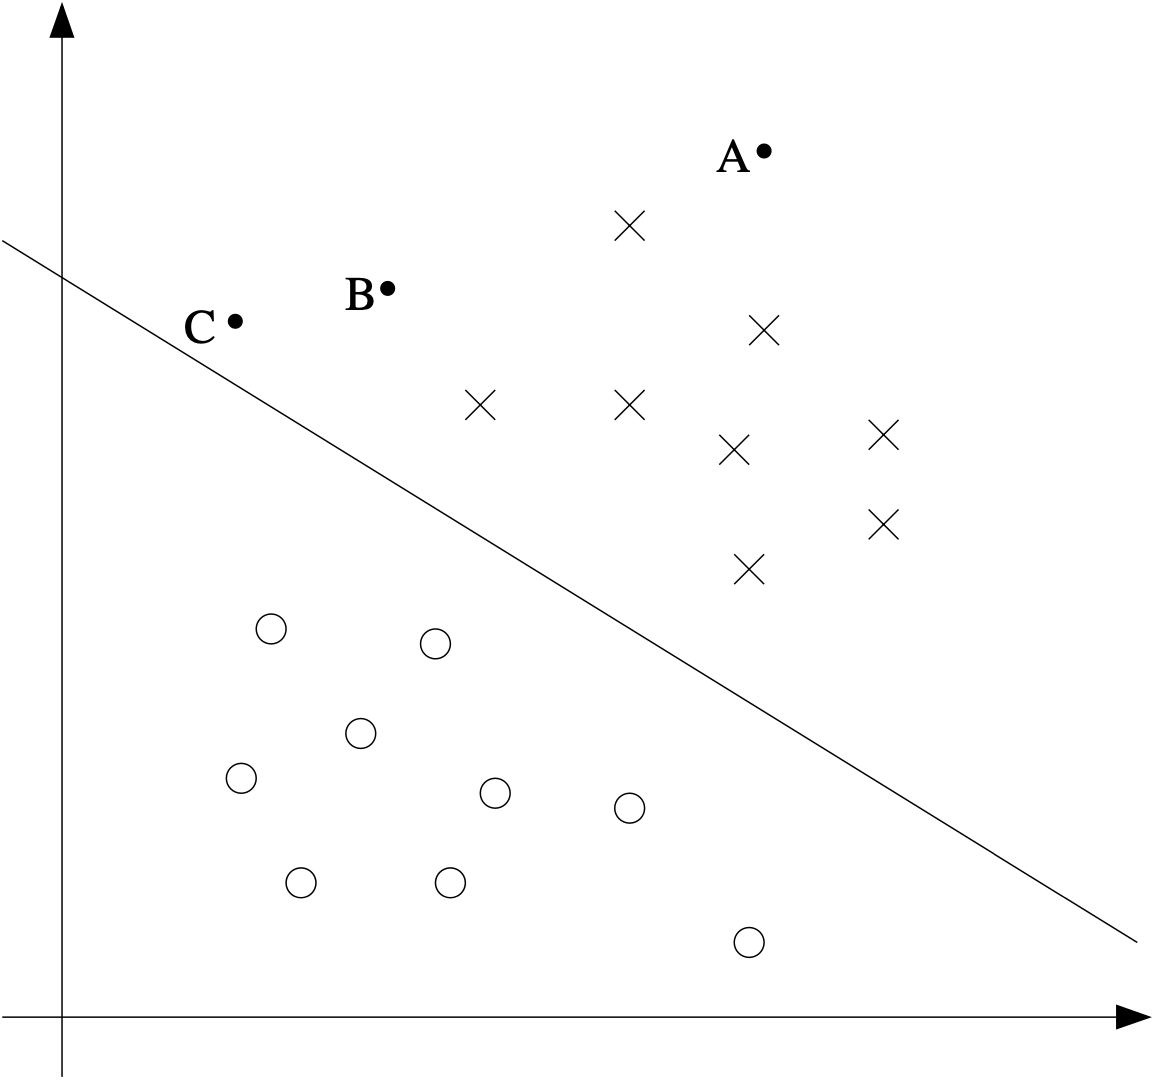
\includegraphics[scale=0.5]{figs/margin.png}
\end{center}

توجه کنید که نقطه‌ی
\lr{A}
بسیار دور از مرز تصمیم قرار دارد. اگر از ما خواسته شود که پیش‌بینی کنیم مقدار
$y$
در
\lr{A}
چقدر است، به نظر می‌رسد که باید بسیار مطمئن باشیم که
$y = 1$
است. برعکس، نقطه‌ی
\lr{C}
بسیار نزدیک به مرز تصمیم قرار دارد، و در حالی که در طرف مرز تصمیم است که ما
$y = 1$
را پیش‌بینی می‌کنیم، به نظر می‌رسد که فقط یک تغییر کوچک در مرز تصمیم به راحتی می‌توانست پیش‌بینی ما را به
$y = 0$
تغییر دهد. بنابراین، ما از پیش‌بینی خود درباره‌ی
\lr{A}
نسبت به
\lr{C}
بسیار مطمئن‌تر هستیم. نقطه‌ی
\lr{B}
در بین این دو مورد قرار دارد و به طور کلی می‌بینیم که اگر نقطه‌ای دور از ابرصفحه‌ی جداکننده باشد، ممکن است به طور قابل توجهی در پیش‌بینی‌های خود مطمئن‌تر باشیم. دوباره به طور غیررسمی فکر می‌کنیم که اگر با توجه به یک مجموعه‌ی آموزشی، مرز تصمیمی پیدا کنیم که به ما اجازه دهد تمام پیش‌بینی‌های درست و مطمئن (به معنای دور از مرز تصمیم) در مثال‌های آموزشی داشته باشیم، این یک امر خوب خواهد بود. این ایده را بعداً با استفاده از مفهوم حاشیه‌های هندسی رسمی خواهیم کرد.

\section{نمادگذاری}
برای آسان‌تر کردن بحثمان درباره‌ی
\lr{SVM}
ها، ابتدا باید یک نمادگذاری جدید برای صحبت درباره‌ی طبقه‌بندی 
(\lr{Classification})
معرفی کنیم. ما یک طبقه‌بند خطی برای مسئله‌ی طبقه‌بندی دودویی با برچسب‌های
$y$
و ویژگی‌های
$x$
در نظر خواهیم گرفت. از این پس، از
$y \in \{-1, 1\}$
به جای
$\{0, 1\}$
برای نشان دادن برچسب‌های کلاس استفاده خواهیم کرد. همچنین به جای پارامتردهی طبقه‌بند خطی‌مان با بردار
$\theta$،
از پارامترهای
$w$
و
$b$
استفاده می‌کنیم و طبقه‌بندمان را به صورت زیر می‌نویسیم
$$h_{w,b}(x) = g(w^T x + b).$$

اینجا،
$g(z) = 1$
اگر
$z \geq 0$
و در غیر این صورت
$g(z) = -1$.
این نمادگذاری
$w$
و
$b$
به ما اجازه می‌دهد که جمله‌ی تقاطع
$b$
را به طور مجزا از سایر پارامترها به صورت صریح در نظر بگیریم (همچنین از این رویه که قبلاً داشتیم که
$x_0 = 1$
باشد به عنوان یک مختصات اضافی در بردار ویژگی ورودی چشم‌پوشی می‌کنیم). بنابراین
$b$
نقش آنچه قبلاً
$\theta_0$
بود را بازی می‌کند، و
$w$
نقش
$[\theta_1 \ldots \theta_d]^T$
را بازی می‌کند.

همچنین توجه کنید که از تعریف
$g$
که در بالا آوردیم، طبقه‌بند ما مستقیماً ۱ یا -۱ را پیش‌بینی می‌کند (مانند الگوریتم
\lr{Perceptron})،
بدون این که ابتدا از مرحله‌ی میانی برآورد
$p(y = 1)$
عبور کند (که این همان کاری است که رگرسیون لجستیک انجام می‌دهد).

\section{حاشیه‌های تابعی و هندسی}
بیایید مفاهیم حاشیه‌های تابعی و هندسی را رسمی کنیم. با در نظر گرفتن یک مثال آموزشی
$(x^{(i)}, y^{(i)})$،
حاشیه‌ی تابعی
$(w, b)$
نسبت به این مثال آموزشی به صورت زیر تعریف می‌شود
$$\hat{\gamma}^{(i)} = y^{(i)} (w^T x^{(i)} + b).$$

توجه کنید که اگر
$y^{(i)} = 1$
باشد، برای اینکه حاشیه‌ی تابعی بزرگ باشد (یعنی پیش‌بینی ما مطمئن و صحیح باشد)، نیاز داریم
$w^T x^{(i)} + b$
عددی بزرگ و مثبت باشد. برعکس، اگر
$y^{(i)} = -1$
باشد، برای اینکه حاشیه‌ی تابعی بزرگ باشد، نیاز داریم
$w^T x^{(i)} + b$
عددی بزرگ و منفی باشد. علاوه بر این، اگر
$y^{(i)} (w^T x^{(i)} + b) > 0$
باشد، پیش‌بینی ما در این مثال صحیح است (خودتان این را بررسی کنید). بنابراین، یک حاشیه‌ی تابعی بزرگ نشان‌دهنده‌ی یک پیش‌بینی مطمئن و صحیح است.

برای یک طبقه‌بند خطی با انتخاب تابع
$g$
که در بالا ذکر شد (که مقادیر
$\{-1, 1\}$
را می‌گیرد)، یک خاصیت حاشیه‌ی تابعی وجود دارد که آن را به عنوان یک معیار اعتماد چندان خوب نمی‌سازد. با توجه به انتخاب تابع
$g$،
توجه می‌کنیم که اگر
$w$
را با
$2w$
و
$b$
را با
$2b$
جایگزین کنیم، از آنجایی که
$g(w^T x + b) = g(2w^T x + 2b)$
است، این هیچ تغییری در
$h_{w,b}(x)$
ایجاد نمی‌کند. به عبارتی،
$g$
و در نتیجه
$h_{w,b}(x)$
تنها به علامت
$w^T x + b$
وابسته هستند، نه به اندازه‌ی آن. اما جایگزینی
$(w, b)$
با
$(2w, 2b)$
همچنین باعث می‌شود که حاشیه‌ی تابعی ما با ضریبی از ۲ ضرب شود. بنابراین، به نظر می‌رسد که با استفاده از آزادی ما در مقیاس‌گذاری
$w$
و
$b$،
می‌توانیم حاشیه‌ی تابعی را به دلخواه بزرگ کنیم بدون اینکه واقعاً چیزی را تغییر دهیم. به طور شهودی، ممکن است منطقی باشد که نوعی شرط نرمال‌سازی مانند
$||w||_2 = 1$
اعمال کنیم؛ یعنی ممکن است
$(w, b)$
را با
$(w/||w||_2, b/||w||_2)$
جایگزین کنیم و به جای آن حاشیه‌ی تابعی
$(w/||w||_2, b/||w||_2)$
را در نظر بگیریم. بعداً به این موضوع بازخواهیم گشت.

با در نظر گرفتن یک مجموعه‌ی آموزشی
$S = \{(x^{(i)}, y^{(i)}); i = 1, \ldots, n\}$،
حاشیه‌ی تابعی
$(w, b)$
نسبت به
$S$
به صورت کوچک‌ترین حاشیه‌ی تابعی مثال‌های آموزشی فردی تعریف می‌شود
$$\hat{\gamma} = \min_{i=1, \ldots, n} \hat{\gamma}^{(i)}.$$

اکنون، بیایید درباره‌ی حاشیه‌های هندسی صحبت کنیم. شکل زیر را در نظر بگیرید:
\begin{center}
    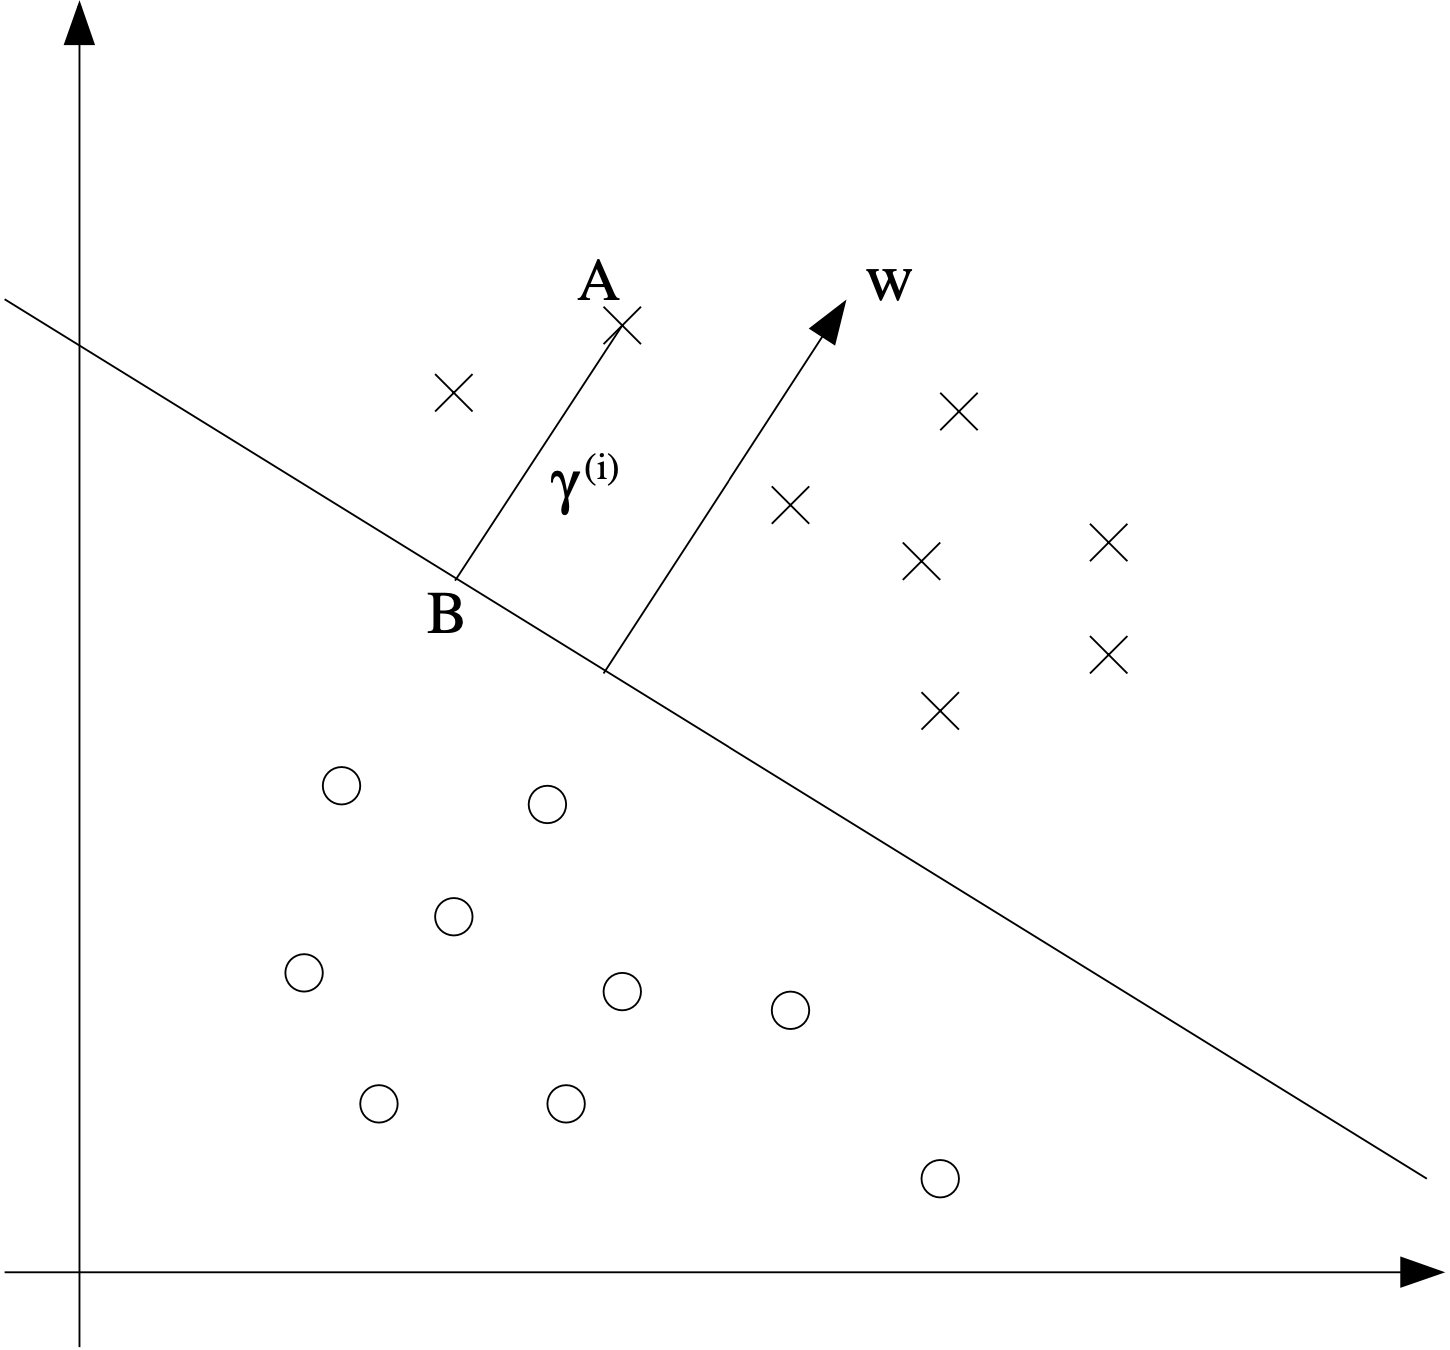
\includegraphics[scale=0.4]{figs/geo-margin.png}
\end{center}

مرز تصمیم متناظر با
$(w, b)$
همراه با بردار
$w$
نشان داده شده است. توجه کنید که
$w$
عمود بر ابرصفحه‌ی جداکننده است (چرا؟). نقطه‌ی
\lr{A}
را در نظر بگیرید که نمایانگر ورودی
$x^{(i)}$
از یک مثال آموزشی با برچسب
$y^{(i)} = 1$
است. فاصله‌ی آن تا مرز تصمیم
$\gamma^{(i)}$
توسط خط
\lr{AB}
داده شده است.

چگونه می‌توانیم مقدار
$\gamma^{(i)}$
را پیدا کنیم؟ همانطور که می‌دانیم
$w/||w||$
یک بردار با طول واحد است که در همان جهت
$w$
اشاره دارد. از آنجا که
\lr{A}
نمایانگر
$x^{(i)}$
است، بنابراین متوجه می‌شویم که نقطه‌ی
\lr{B}
به صورت
$x^{(i)} - \gamma^{(i)} \cdot w/||w||$
داده می‌شود. اما این نقطه بر روی مرز تصمیم قرار دارد، و تمام نقاط
$x$
روی مرز تصمیم معادله‌ی
$w^T x + b = 0$
را ارضا می‌کنند. بنابراین،
$$w^T \left( x^{(i)} - \gamma^{(i)} \frac{w}{||w||} \right) + b = 0.$$

با حل کردن برای
$\gamma^{(i)}$
به دست می‌آوریم
$$\gamma^{(i)} = \frac{w^T x^{(i)} + b}{||w||} = \left( \frac{w}{||w||} \right)^T x^{(i)} + \frac{b}{||w||}.$$

این برای حالتی که یک مثال آموزشی مثبت
\lr{A}
در شکل داریم که در طرف مثبت مرز تصمیم است خوب است. به طور کلی، حاشیه‌ی هندسی
$(w, b)$
نسبت به یک مثال آموزشی
$(x^{(i)}, y^{(i)})$
به صورت زیر تعریف می‌شود
$$\gamma^{(i)} = y^{(i)} \left( \left( \frac{w}{||w||} \right)^T x^{(i)} + \frac{b}{||w||} \right).$$

توجه کنید که اگر
$||w|| = 1$
باشد، حاشیه‌ی تابعی برابر با حاشیه‌ی هندسی است - این به ما راهی برای مرتبط کردن این دو مفهوم متفاوت از حاشیه می‌دهد. همچنین، حاشیه‌ی هندسی نسبت به مقیاس‌بندی پارامترها نامتغیر است؛ یعنی، اگر
$w$
را با
$2w$
و
$b$
را با
$2b$
جایگزین کنیم، حاشیه‌ی هندسی تغییر نمی‌کند. این موضوع در آینده به کار خواهد آمد. به طور خاص، به دلیل این نامتغیری نسبت به مقیاس‌بندی پارامترها، وقتی سعی می‌کنیم
$w$
و
$b$
را به داده‌های آموزشی برازش دهیم، می‌توانیم یک محدودیت مقیاس‌بندی دلخواه بر
$w$
اعمال کنیم بدون اینکه چیزی مهم را تغییر دهیم؛ به عنوان مثال، می‌توانیم بگوییم
$||w|| = 1$
یا
$|w_1| = 5$
یا
$|w_1 + b| + |w_2| = 2$
و هر یک از این‌ها را می‌توانیم به سادگی با مقیاس‌بندی مجدد
$w$
و
$b$
ارضا کنیم.

در نهایت، با در نظر گرفتن یک مجموعه‌ی آموزشی
$S = \{(x^{(i)}, y^{(i)}); i = 1, \ldots, n\}$،
حاشیه‌ی هندسی
$(w, b)$
نسبت به
$S$
به صورت کوچک‌ترین حاشیه‌های هندسی مثال‌های آموزشی فردی تعریف می‌شود
$$\gamma = \min_{i=1, \ldots, n} \gamma^{(i)}.$$

\section{طبقه‌بند حاشیه‌ی بهینه}
با توجه به یک مجموعه‌ی آموزشی، از بحث قبلی ما به نظر می‌رسد که یک مطلوبیت طبیعی این است که سعی کنیم یک مرز تصمیم پیدا کنیم که حاشیه‌ی هندسی را به حداکثر برساند، زیرا این بازتاب‌دهنده‌ی یک مجموعه پیش‌بینی بسیار مطمئن بر روی مجموعه‌ی آموزشی و یک برازش خوب برای داده‌های آموزشی است. به طور خاص، این نتیجه یک طبقه‌بند خواهد داشت که مثال‌های آموزشی مثبت و منفی را با یک فاصله (حاشیه‌ی هندسی) جدا می‌کند.

فعلاً فرض می‌کنیم که یک مجموعه‌ی آموزشی داده شده که به صورت خطی جداپذیر است؛ یعنی، امکان جدا کردن مثال‌های مثبت و منفی با استفاده از یک ابرصفحه‌ی جداکننده وجود دارد. چگونه می‌توانیم یکی را پیدا کنیم که حداکثر حاشیه‌ی هندسی را بدست آورد؟ می‌توانیم مسئله‌ی بهینه‌سازی زیر را مطرح کنیم
\begin{align*}
    \max_{\gamma, w, b}\hspace{4} & \gamma \\
    \text{\lr{s.t. }} & y^{(i)}(w^T x^{(i)} + b) \geq \gamma, \quad i = 1, \ldots, n \\
    & ||w|| = 1.
\end{align*}

یعنی می‌خواهیم
$\gamma$
را به حداکثر برسانیم، به شرطی که هر مثال آموزشی حاشیه‌ی تابعی حداقل
$\gamma$
داشته باشد. همچنین قید
$||w|| = 1$
اطمینان می‌دهد که حاشیه‌ی تابعی برابر با حاشیه‌ی هندسی است. بنابراین تضمین می‌شود که تمام حاشیه‌های هندسی حداقل
$\gamma$
هستند. بنابراین حل این مسئله منجر به
$(w, b)$
با حداکثر حاشیه‌ی هندسی ممکن نسبت به مجموعه آموزشی خواهد شد.

اگر بتوانیم مسئله بهینه‌سازی بالا را حل کنیم، کارمان تمام است. اما قید
$||w|| = 1$
یک قید ناخوشایند (غیرمحدب) است، و این مسئله قطعاً در هیچ فرمتی نیست که بتوانیم به نرم‌افزارهای بهینه‌سازی استاندارد وصل کنیم تا حل شود. بنابراین، بیایید سعی کنیم مسئله را به یک مسئله‌ی خوشایندتر تبدیل کنیم. در نظر بگیرید:
\begin{align*}
    \max_{\hat{\gamma}, w, b}\hspace{4} & \frac{\hat{\gamma}}{||w||} \\
    \text{\lr{s.t. }} & y^{(i)}(w^T x^{(i)} + b) \geq \hat{\gamma}, \quad i = 1, \ldots, n
\end{align*}

اینجا می‌خواهیم
$\frac{\hat{\gamma}}{||w||}$
را به حداکثر برسانیم، به شرطی که تمام حاشیه‌های تابعی حداقل
$\hat{\gamma}$
باشند. از آنجایی که حاشیه‌های هندسی و تابعی توسط
$\gamma = \frac{\hat{\gamma}}{||w||}$
مرتبط هستند، این همان جوابی را که می‌خواهیم به ما می‌دهد. علاوه بر این، از قید
$||w|| = 1$
که دوست نداشتیم خلاص شده‌ایم. نقطه ضعف این است که اکنون یک تابع هدف ناخوشایند (دوباره غیرمحدب)
$\frac{\hat{\gamma}}{||w||}$
داریم و هنوز هیچ نرم‌افزار آماده‌ای نداریم که بتواند این فرم از مسئله‌ی بهینه‌سازی را حل کند.

بحث قبلی ما را به خاطر بیاورید که می‌توانیم یک قید مقیاس‌بندی دلخواه بر
$w$
و
$b$
اضافه کنیم بدون اینکه چیزی را تغییر دهیم. این ایده‌ی کلیدی است که اکنون از آن استفاده خواهیم کرد. قید مقیاس‌بندی که حاشیه‌ی تابعی
$w, b$
نسبت به مجموعه‌ی آموزشی باید ۱ باشد را معرفی می‌کنیم:
$$\hat{\gamma} = 1.$$

از آنجایی که ضرب کردن
$w$
و
$b$
در یک ثابت باعث می‌شود حاشیه‌ی تابعی با همان ثابت ضرب شود، این قطعاً یک قید مقیاس‌بندی است و می‌توان با مقیاس‌بندی مجدد
$w, b$
آن را ارضا کرد. با جایگذاری این در مسئله‌ی بالا و با توجه به اینکه حداکثر کردن
$\frac{\hat{\gamma}}{||w||} = \frac{1}{||w||}$
همان چیزی است که حداقل کردن
$||w||^2$
است، اکنون مسئله‌ی بهینه‌سازی زیر را داریم:
\begin{align*}
    \min_{w, b}\hspace{4} & \frac{1}{2} ||w||^2 \\
    \text{\lr{s.t. }} & y^{(i)}(w^T x^{(i)} + b) \geq 1, \quad i = 1, \ldots, n
\end{align*}

ما اکنون مسئله را به شکلی تبدیل کرده‌ایم که می‌تواند به طور کارآمد حل شود. مسئله‌ی بالا یک مسئله‌ی بهینه‌سازی با یک تابع هدف درجه دوم محدب و تنها قیود خطی است. حل آن طبقه‌بند حاشیه‌ی بهینه را به ما می‌دهد. این مسئله‌ی بهینه‌سازی را می‌توان با استفاده از کدهای برنامه‌ریزی درجه دوم تجاری
(\lr{QP})
حل کرد.

در حالی که می‌توانستیم مسئله را اینجا حل‌شده در نظر بگیریم، کاری که در عوض انجام خواهیم داد این است که به بحثی در مورد دوگان لاگرانژ
(\lr{Lagrange duality})
بپردازیم. این ما را به فرم دوگان مسئله بهینه‌سازی‌مان هدایت خواهد کرد که نقش کلیدی در استفاده از هسته‌ها برای به‌کارگیری طبقه‌بندهای حاشیه‌ی بهینه به طور کارآمد در فضاهای با ابعاد بسیار بالا خواهد داشت. فرم دوگان همچنین به ما امکان می‌دهد تا الگوریتمی کارآمد برای حل مسئله‌ی بهینه‌سازی بالا به دست آوریم که به طور معمول بهتر از نرم‌افزار
\lr{QP}
عمومی عمل خواهد کرد.

\section{دوگان لاگرانژ}
بیایید به طور موقت از
\lr{SVM}
ها و طبقه‌بندهای حاشیه‌ی بهینه فاصله بگیریم و درباره‌ی حل مسائل بهینه‌سازی با قیود صحبت کنیم.

یک مسئله از فرم زیر را در نظر بگیرید
\begin{align*}
    \min_{w}\hspace{4} & f(w) \\
    \text{\lr{s.t. }} & h_i(w) = 0, \quad i = 1, \ldots, l.
\end{align*}

برخی از شما ممکن است به یاد بیاورید که چگونه روش ضرایب لاگرانژ 
(\lr{Lagrange multipliers})
می‌تواند برای حل آن استفاده شود (اگر قبلاً آن را ندیده‌اید نگران نباشید). در این روش، لاگرانژی به صورت زیر تعریف می‌شود:
$$L(w, \beta) = f(w) + \sum_{i=1}^l \beta_i h_i(w)$$

در اینجا،
$\beta_i$
ها ضرایب لاگرانژ نامیده می‌شوند. سپس مشتقات جزئی
$L$
را پیدا کرده و آن‌ها را برابر با صفر قرار می‌دهیم:
$$\frac{\partial L}{\partial w_i} = 0, \quad \frac{\partial L}{\partial \beta_i} = 0$$
و برای
$w$
و
$\beta$
حل می‌کنیم.

در این بخش، این مفهوم را به مسائل بهینه‌سازی با قیود نامساوی و مساوی گسترش خواهیم داد. به دلیل محدودیت‌های زمانی، واقعاً نمی‌توانیم نظریه دوگان لاگرانژ را در این کلاس به درستی پوشش دهیم، اما ایده‌ها و نتایج اصلی را ارائه خواهیم داد که سپس آن‌ها را به مسئله‌ی بهینه‌سازی طبقه‌بند حاشیه‌ی بهینه‌ی خود اعمال خواهیم کرد.

مسئله‌ی زیر را در نظر بگیرید که آن را مسئله‌ی بهینه‌سازی اولیه
(\lr{Primal optimization problem})
می‌نامیم
\begin{align*}
    \min_{w}\hspace{4} & f(w) \\
    \text{\lr{s.t. }} & g_i(w) \leq 0, \quad i = 1, \ldots, k \\
    & h_i(w) = 0, \quad i = 1, \ldots, l.
\end{align*}

برای حل آن با تعریف لاگرانژی عمومی شروع می‌کنیم:
$$L(w, \alpha, \beta) = f(w) + \sum_{i=1}^k \alpha_i g_i(w) + \sum_{i=1}^l \beta_i h_i(w).$$

در اینجا
$\alpha_i$
ها و
$\beta_i$
ها ضرایب لاگرانژ هستند. مقدار زیر را در نظر بگیرید
$$\theta_P(w) = \max_{\alpha, \beta : \alpha_i \geq 0} L(w, \alpha, \beta).$$

در اینجا، زیرنویس
$P$
به معنای اولیه
(\lr{Primal})
است. فرض کنید
$w$
داده شده باشد. اگر
$w$
هرکدام از قیود اولیه را نقض کند (یعنی
$g_i(w) > 0$
یا
$h_i(w) \neq 0$
برای یکی از
$i$
ها)
می‌توانید تأیید کنید که
$$\theta_P(w) = \max_{\alpha, \beta : \alpha_i \geq 0} \left[ f(w) + \sum_{i=1}^k \alpha_i g_i(w) + \sum_{i=1}^l \beta_i h_i(w) \right] = \infty.$$

برعکس، اگر قیود واقعاً برای یک مقدار خاص از
$w$
ارضا شوند، آنگاه
$\theta_P(w) = f(w)$.
بنابراین،
$$
\theta_P(w) = 
\begin{cases}
f(w) & \text{\lr{if }} w \text{\lr{ satisfies primal constraints}} \\
\infty & \text{\lr{otherwise}}.
\end{cases}
$$

بنابراین
$\theta_P$
همان مقدار هدف مسئله ما را برای تمام مقادیر
$w$
که قیود اولیه را ارضا می‌کنند می‌گیرد، و اگر قیود نقض شوند، بی‌نهایت می‌شود. بنابراین، اگر مسئله‌ی حداقل‌سازی زیر را در نظر بگیریم
$$\min_{w} \theta_P(w) = \min_{w} \max_{\alpha, \beta : \alpha_i \geq 0} L(w, \alpha, \beta),$$

می‌بینیم که این همان مسئله‌ی اولیه‌ی ما است (و همان راه‌حل‌ها را دارد). برای استفاده‌های بعدی، مقدار بهینه‌ی هدف را
$p^* = \min_{w} \theta_P(w)$
تعریف می‌کنیم؛ این را مقدار مسئله‌ی اولیه می‌نامیم.

اکنون به مسئله‌ای کمی متفاوت‌تر نگاه می‌کنیم
$$\theta_D(\alpha, \beta) = \min_{w} L(w, \alpha, \beta).$$

در اینجا، زیرنویس
\lr{D}
به معنای دوگان است. همچنین توجه کنید که در تعریف
$\theta_P$،
ما با توجه به
$\alpha, \beta$
بهینه‌سازی (حداکثر) می‌کردیم، اما در اینجا با توجه به
$w$
بهینه‌سازی (حداقل) می‌کنیم.

اکنون می‌توانیم مسئله‌ی بهینه‌سازی دوگان را مطرح کنیم:
$$\max_{\alpha, \beta : \alpha_i \geq 0} \theta_D(\alpha, \beta) = \max_{\alpha, \beta : \alpha_i \geq 0} \min_{w} L(w, \alpha, \beta).$$

این دقیقاً همان مسئله‌ی اولیه‌ی ما است که در بالا نشان داده شده، با این تفاوت که ترتیب
\lr{max}
و
\lr{min}
تغییر کرده است. همچنین مقدار بهینه‌ی هدف مسئله‌ی دوگان را
$d^* = \max_{\alpha, \beta : \alpha_i \geq 0} \theta_D(w)$
تعریف می‌کنیم.

چگونه مسائل اولیه و دوگان مرتبط هستند؟ می‌توان به راحتی نشان داد که
$$d^* = \max_{\alpha, \beta : \alpha_i \geq 0} \min_{w} L(w, \alpha, \beta) \leq \min_{w} \max_{\alpha, \beta : \alpha_i \geq 0} L(w, \alpha, \beta) = p^*.$$

باید خودتان را متقاعد کنید که این درست است؛ زیرا از شرط همواره کمتر یا مساوی بودن
\lr{maxmin}
یک تابع از
\lr{minmax}
آن پیروی می‌کند. اما تحت شرایط خاصی خواهیم داشت
$$d^* = p^*.$$

بنابراین می‌توانیم مسئله‌ی دوگان را به جای مسئله‌ی اولیه حل کنیم. بیایید ببینیم این شرایط چیست.

فرض کنید
$f$
و
$g_i$
ها محدب هستند و
$h_i$
ها خطی هستند. همچنین فرض کنید که قیود
$g_i$
نیز (به طور دقیق) قابل ارضا هستند؛ این به این معناست که
$w$
ای وجود دارد که برای تمام
$i$
ها، شرط
$g_i(w) < 0$
برقرار است.

تحت فرضیات بالا، باید
$w^*, \alpha^*, \beta^*$
وجود داشته باشد، به طوری که
$w^*$
راه‌حل مسئله‌ی اولیه باشد،
$\alpha^*, \beta^*$
راه‌حل مسئله‌ی دوگان باشند و همچنین
$p^* = d^* = L(w^*, \alpha^*, \beta^*)$.
علاوه بر این
$w^*, \alpha^*$
و
$\beta^*$
شرایط
\lr{KKT}
را ارضا می‌کنند، که به شرح زیر است
\begin{align*}
    \frac{\partial L}{\partial w_i}(w^*, \alpha^*, \beta^*) &= 0, \quad i = 1, \ldots, d \\
    \frac{\partial L}{\partial \beta_i}(w^*, \alpha^*, \beta^*) &= 0, \quad i = 1, \ldots, l \\
    \alpha^*_i g_i(w^*) &= 0, \quad i = 1, \ldots, k \\
    g_i(w^*) &\leq 0, \quad i = 1, \ldots, k \\
    \alpha^*_i &\geq 0, \quad i = 1, \ldots, k.
\end{align*}

علاوه بر این، اگر یک مجموعه‌ی
$w^*, \alpha^*, \beta^*$
شرایط
\lr{KKT}
را ارضا کنند، آن‌ها نیز یک راه‌حل برای مسائل اولیه و دوگان هستند.

به شرط سوم توجه می‌کنیم که به آن شرط مکمل دوگان
\lr{KKT}
گفته می‌شود. به طور خاص، این به معنای آن است که اگر
$\alpha^*_i > 0$،
آنگاه
$g_i(w^*) = 0$
(یعنی، قید
$g_i(w) \leq 0$
فعال است، به این معنی که با برابری نگه داشته می‌شود نه با نابرابری). بعداً این کلید نشان دادن این خواهد بود که
\lr{SVM}
تنها تعداد کمی بردار پشتیبانی دارد؛ شرط مکمل دوگان
\lr{KKT}
همچنین آزمون همگرایی ما را زمانی که درباره‌ی الگوریتم
\lr{SMO}
صحبت می‌کنیم، فراهم می‌کند.

\section{طبقه‌بندهای حاشیه‌ی بهینه: فرم دوگان}
قبلاً مسئله‌ی بهینه‌سازی (اولیه) زیر را برای یافتن طبقه‌بند حاشیه‌ی بهینه مطرح کرده بودیم:
\begin{align*}
    \min_{w, b}\hspace{4} &\frac{1}{2} ||w||^2 \\
    \text{\lr{s.t. }} & y^{(i)}(w^T x^{(i)} + b) \geq 1, \quad i = 1, \ldots, n
\end{align*}

می‌توانیم قیود را به صورت زیر بنویسیم
$$g_i(w) = -y^{(i)}(w^T x^{(i)} + b) + 1 \leq 0.$$

برای هر مثال آموزشی یک قید داریم. توجه کنید که از شرط مکمل دوگان
\lr{KKT}،
فقط برای مثال‌های آموزشی که حاشیه‌ی تابعی دقیقاً برابر با یک دارند، خواهیم داشت
$\alpha_i > 0$
(یعنی
$i$
هایی که متناظر با قیودی هستند که با برابری نگه داشته می‌شوند
$g_i(w) = 0$).
شکل زیر را در نظر بگیرید که در آن یک صفحه‌ی جداکننده با حداکثر حاشیه با خط ممتد نشان داده شده است:
\begin{center}
    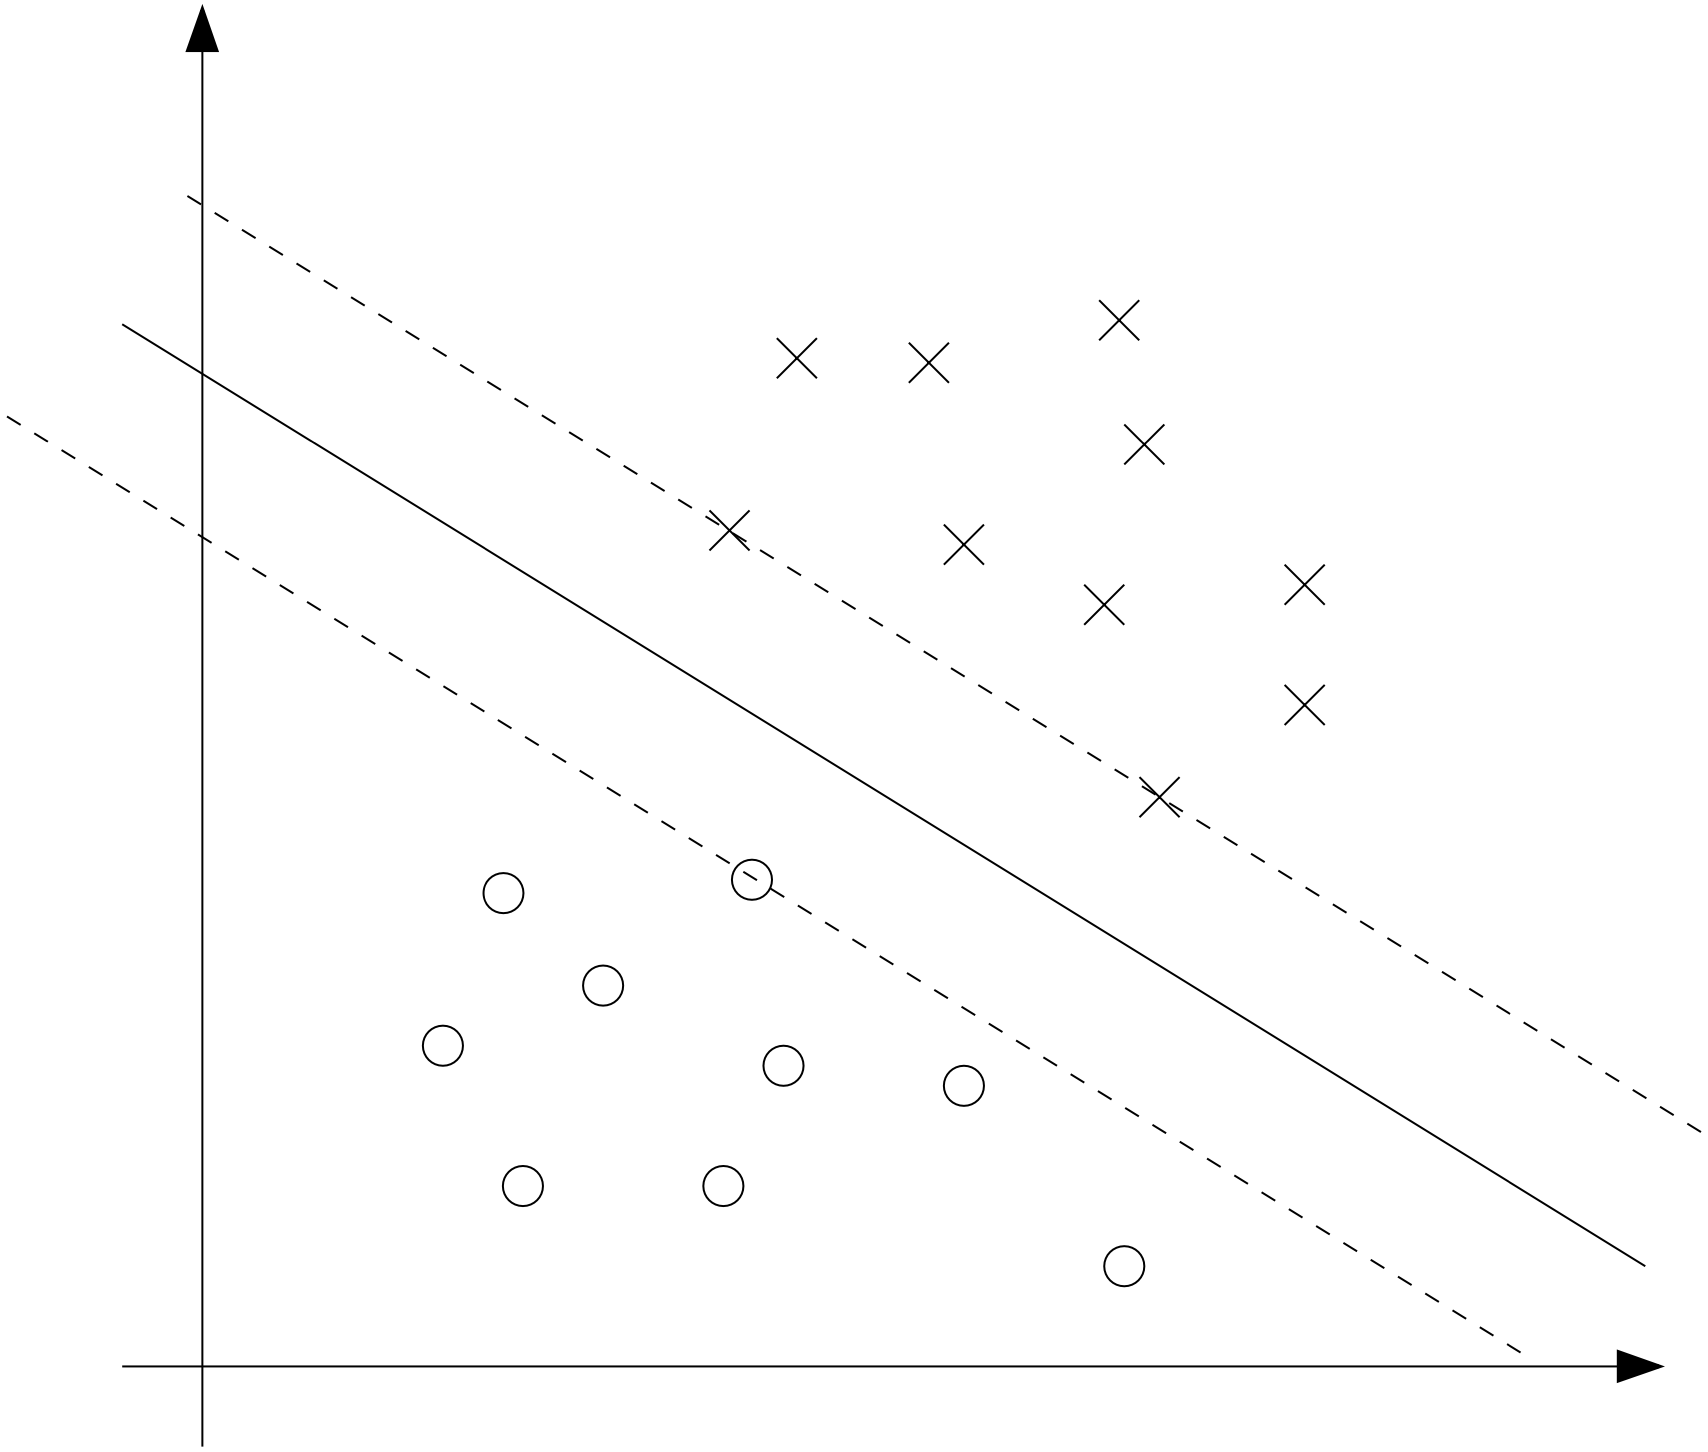
\includegraphics[scale=0.4]{figs/max-margin.png}
\end{center}

نقاط با کوچکترین حاشیه‌ها دقیقاً همان‌هایی هستند که نزدیک‌ترین به مرز تصمیم هستند؛ در اینجا، این‌ها سه نقطه (یک مثال منفی و دو مثال مثبت) هستند که روی خطوط خط‌چین موازی با مرز تصمیم قرار دارند. بنابراین، فقط سه
$\alpha_i$
- یعنی آن‌هایی که متناظر با این سه مثال آموزشی هستند - در راه‌حل بهینه‌ی مسئله‌ی بهینه‌سازی ما غیرصفر خواهند بود. این سه نقطه در این مسئله بردارهای پشتیبانی نامیده می‌شوند. این که تعداد بردارهای پشتیبانی می‌تواند بسیار کمتر از اندازه مجموعه‌ی آموزشی باشد، بعداً مفید خواهد بود.

هنگامی که فرم دوگان مسئله را توسعه می‌دهیم، یکی از ایده‌های کلیدی که باید به آن توجه کنیم این است که سعی می‌کنیم الگوریتم خود را فقط بر حسب حاصل‌ضرب داخلی
$\langle x^{(i)}, x^{(j)} \rangle$
(این را به صورت
$(x^{(i)})^T x^{(j)}$
در نظر بگیرید) بین نقاط در فضای ویژگی ورودی بنویسیم. این که می‌توانیم الگوریتم خود را بر حسب این حاصل‌ضرب‌های داخلی بیان کنیم، زمانی که ترفند هسته
(\lr{Kernel trick})
را اعمال کنیم، کلیدی خواهد بود.

وقتی لاگرانژی برای مسئله‌ی بهینه‌سازی خود ساختیم، داریم
$$L(w, b, \alpha) = \frac{1}{2} ||w||^2 - \sum_{i=1}^n \alpha_i [y^{(i)}(w^T x^{(i)} + b) - 1].$$

توجه کنید که فقط
$\alpha_i$
داریم و هیچ ضریب
$\beta_i$
لاگرانژ وجود ندارد، زیرا مسئله فقط قیود نامساوی دارد.

بیایید فرم دوگان مسئله را پیدا کنیم. برای انجام این کار ابتدا باید
$L(w, b, \alpha)$
را با توجه به
$w$
و
$b$
(برای
$\alpha$
ثابت) به حداقل برسانیم تا
$\theta_D$
را به دست آوریم که با قرار دادن مشتقات
$L$
نسبت به
$w$
و
$b$
برابر صفر انجام می‌دهیم. داریم:
$$\nabla_w L(w, b, \alpha) = w - \sum_{i=1}^n \alpha_i y^{(i)} x^{(i)} = 0$$

این به این معناست که
$$w = \sum_{i=1}^n \alpha_i y^{(i)} x^{(i)}.$$

همچنین، برای مشتق نسبت به $b$، داریم
$$\frac{\partial L}{\partial b} = \sum_{i=1}^n \alpha_i y^{(i)} = 0.$$

اگر تعریف
$w$
در معادله‌ی آن را بگیریم و آن را دوباره در لاگرانژی جایگذاری کنیم و ساده‌سازی کنیم، داریم
$$L(w, b, \alpha) = \sum_{i=1}^n \alpha_i - \frac{1}{2} \sum_{i,j=1}^n y^{(i)} y^{(j)} \alpha_i \alpha_j (x^{(i)})^T x^{(j)} - b \sum_{i=1}^n \alpha_i y^{(i)}.$$

اما از معادله‌ی گرادیان‌ها، جمله‌ی آخر باید صفر باشد، بنابراین داریم
$$L(w, b, \alpha) = \sum_{i=1}^n \alpha_i - \frac{1}{2} \sum_{i,j=1}^n y^{(i)} y^{(j)} \alpha_i \alpha_j (x^{(i)})^T x^{(j)}.$$

به یاد داشته باشید که با حداقل‌سازی
$L$
با توجه به
$w$
و
$b$
به معادله‌ی بالا رسیدیم. با قرار دادن این به همراه قیود
$\alpha_i \geq 0$
(که همیشه داشتیم) و قید گرادیان‌ها، مسئله‌ی بهینه‌سازی دوگان زیر را داریم
\begin{align*}
    \max_{\alpha}\hspace{4} & W(\alpha) = \sum_{i=1}^n \alpha_i - \frac{1}{2} \sum_{i,j=1}^n y^{(i)} y^{(j)} \alpha_i \alpha_j \langle x^{(i)}, x^{(j)} \rangle \\
    \text{\lr{s.t. }} & \alpha_i \geq 0, \quad i = 1, \ldots, n \\
    & \sum_{i=1}^n \alpha_i y^{(i)} = 0.
\end{align*}

همچنین باید بتوانید تأیید کنید که شرایط لازم برای
$p^* = d^*$
و شرایط
\lr{KKT}
در مسئله‌ی بهینه‌سازی ما ارضا می‌شوند. بنابراین، می‌توانیم مسئله دوگان را به جای حل مسئله اولیه حل کنیم. به طور خاص، در مسئله دوگان بالا، یک مسئله به حداکثر رساندن داریم که پارامترهای آن
$\alpha_i$
هستند. بعداً درباره‌ی الگوریتم خاصی که قرار است برای حل مسئله دوگان استفاده کنیم صحبت خواهیم کرد، اما اگر واقعاً بتوانیم آن را حل کنیم (یعنی
$\alpha$
هایی که
$W(\alpha)$
را تحت قیود حداکثر می‌کنند پیدا کنیم)، سپس می‌توانیم از معادله‌ی
$w$
استفاده کنیم و
$w$
های بهینه را به عنوان تابعی از
$\alpha$
ها پیدا کنیم. با پیدا کردن
$w^*$،
با در نظر گرفتن مسئله‌ی اولیه، یافتن مقدار بهینه برای جمله‌ی تقاطع
$b$
نیز ساده است
$$b^* = -\frac{\max_{i: y^{(i)} = -1} w^T x^{(i)} + \min_{i: y^{(i)} = 1} w^T x^{(i)}}{2}.$$

(خودتان بررسی کنید که این درست است.)قبل از ادامه، بیایید نگاهی دقیق‌تر به معادله‌ی
$w$
بیندازیم که مقدار بهینه‌ی
$w$
را به صورت (مقدار بهینه)
$\alpha$
بیان می‌کند. فرض کنید پارامترهای مدل خود را به یک مجموعه‌ی آموزشی برازش داده‌ایم و اکنون می‌خواهیم در یک نقطه‌ی ورودی جدید
$x$
پیش‌بینی کنیم. سپس
$w^T x + b$
را محاسبه کرده و
$y = 1$
را پیش‌بینی می‌کنیم اگر و فقط اگر این مقدار بزرگتر از صفر باشد. اما با استفاده از این معادله، این مقدار را نیز می‌توان به صورت زیر نوشت
\begin{align*}
    w^T x + b &= \left( \sum_{i=1}^n \alpha_i y^{(i)} x^{(i)} \right)^T x + b \\
    &= \sum_{i=1}^n \alpha_i y^{(i)} \langle x^{(i)}, x \rangle + b.
\end{align*}

بنابراین، اگر
$\alpha_i$
ها را پیدا کرده‌ایم، برای انجام پیش‌بینی باید مقداری را محاسبه کنیم که فقط به حاصل‌ضرب داخلی بین
$x$
و نقاط در مجموعه‌ی آموزشی بستگی دارد. علاوه بر این، قبلاً دیدیم که
$\alpha_i$
ها به جز برای بردارهای پشتیبانی صفر خواهند بود. بنابراین، بسیاری از جملات در مجموع بالا صفر خواهند بود، و واقعاً باید فقط حاصل‌ضرب‌های داخلی بین
$x$
و بردارهای پشتیبانی (که اغلب تعداد کمی دارند) را محاسبه و پیش‌بینی خود را انجام دهیم.

با بررسی فرم دوگان مسئله‌ی بهینه‌سازی، بینش قابل‌توجهی در ساختار مسئله به دست آوردیم، و همچنین توانستیم کل الگوریتم را بر حسب تنها حاصل‌ضرب‌های داخلی بین بردارهای ویژگی ورودی بنویسیم. در بخش‌های بعدی، از این ویژگی برای اعمال هسته‌ها به مسئله‌ی طبقه‌بندی خود استفاده خواهیم کرد. الگوریتم حاصل، ماشین‌های بردار پشتیبانی
(\lr{SVM})،
قادر خواهد بود که به طور کارآمد در فضاهای با ابعاد بسیار بالا یاد بگیرد.
\end{document}